\documentclass[../m2r-report.tex]{subfile}

\subsection{Ramsey's Theorem}
\label{sec:1.1}

Whilst Ramsey's original paper \cite{Ramsey1930} concerned with a problem of logic, Erd{\"o}s and 
Szekeres \cite{Erdos1935} reformulated his work in a graph theoretic sense. The idea of proving 
the existence of regular substructure within an apparently chaotic superstructure
is immediately applicable to graphs. The content of this section primarily follows 
that of Bollobas book \textit{Modern Graph Theory} \cite{Bollobas1998}, and 
I will be using his notation throughout.\\

In the graph below, we partition the edges into two disjoint classes: dotted lines and dashed 
lines. In turns out that no matter how we partition our edges, we will always get
dotted triangles or dashed triangles. In this particular partition, we get two 
dashed triangles.
%The statement in the introduction - ``Given 6 people, either 3 mutually know each
%other, or 3 do not" - can be rephrased in a graph theoretic sense.
%We identify a person with a vertex of the graph, and a relation between them as
%an edge.
%A relation between two people can have  two states: either the two know each other,
%or they have never met.
%We can illustrate this relation status by `colouring' the edge, with a red edge
%showing that the two know each other, and a blue edge showing that they haven't.
%Hence, the situation described by the statement is shown by the following graph:

\begin{figure}[h]
\begin{center}
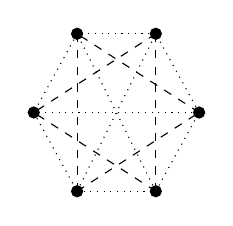
\begin{tikzpicture}
    \draw [dotted] (0,0) -- (1,0);
    \draw [dotted] (1,0) -- (1.55,1);
    \draw [dotted] (1.55,1) -- (1,2);
    \draw [dotted] (1,2) -- (0,2);
    \draw [dotted] (0,2) -- (-0.55,1);
    \draw [dotted] (-0.55,1) -- (0,0);
    \draw [dotted] (0,0) -- (1,2);
    \draw [dotted] (1.55,1) -- (-0.55,1);
    \draw [dotted] (1,0) -- (0,2);
    \draw [dashed] (0,0) -- (0,2);
    \draw [dashed] (1,0) -- (1,2);
    \draw [dashed] (1,0) -- (-0.55,1);
    \draw [dashed] (1.55,1) -- (0,2);
    \draw [dashed] (1,2) -- (-0.55,1);
    \draw [dashed] (0,0) -- (1.55,1);

    \filldraw (0,0) circle (2pt);
    \filldraw (1,0) circle (2pt);
    \filldraw (-0.55,1) circle (2pt);
    \filldraw (1.55,1) circle (2pt);
    \filldraw (0,2) circle (2pt);
    \filldraw (1,2) circle (2pt);

\end{tikzpicture}
\caption{2 dashed triangles within a graph of 6 vertices}
\end{center}
\end{figure}.

Before continuing, we first need to state some notation and definitions.\\ \cite{Graham1990}

For $n,k\in \mathbb{N}$, and any non-empty set $X$, let

\begin{align}
[n] &= \{1, 2,\ldots, n\},
X^{(k)} &= \{Y:Y\subseteq X, |Y|=k\}.
\end{align}
\begin{definition}[Graph]

    A \textit{graph G} is an ordered pair of disjoint sets $(V,E)$ such that $E$ 
    is a subset of $V^{(2)}$, the set of unordered pairs of $V$. We call $V$ the 
    set of vertices, and $E$ the set of edges. The \textit{order}
    of $G$ is the number of vertices, i.e $|V|$.

\end{definition}

\begin{definition}[Complete graph]

    We say a graph $G:=(V,E)$ is \textit{complete} if $E=V^{(2)}$. Intuitively, a graph 
    is complete if every pair of vertices has an edge connecting them. We denoted the complete 
    graph of order $n$ by $K_n$.

\end{definition}

\begin{definition}[Subgraphs and Cliques]

    We say $G':=(V',E')$ is a \textit{subgraph} of $G:=(V,E)$ if $V'\subseteq V$, 
    and $E'\subseteq E$. We write $G'\subseteq G$. We say $G'$ is an \textit{induced} 
    subgraph of $G$ if $E'=E\cap V'^{(2)}$. We say an induced subgraph $G'$ a \textit{clique} of $G$ if it is complete.

\end{definition}

Earlier we mentioned partitioning the edges into disjoint classes. We can think 
of these classes as being `colourings' of the edges. In an \textit{r-colouring}, 
we partition our edges into $r$ disjoint classes, called \textit{colours}. The 
following definition helps explain this:

\begin{definition}[Colouring]
    
    An \textit{r-colouring} of the edges of a graph $G=(V,E)$ is a map \cite{Graham1990}:

    $$\chi : E \rightarrow [r]$$

    We say a subgraph $G' = (V',E')$ of $G$ is \textit{monochromatic} if the restriction
    $\chi|_{E'}$ is the constant map.

\end{definition}

\begin{definition}[Colouring of a set]
    Let $X$ be a non-empty set. For $k\in\mathbb{N}$, a $k$-colouring of $X$ is a 
    partition of $X$ into $k$ equivalence classes. 
    \end{definition}
    
    Equivalently, a $k$-colouring of $X$ is the partition of $X$ induced by an 
    arbitrary map: $$\chi: X \to [k]$$ through the equivalence relation: 
    $$\mathcal{R}_{\chi}:= \{(x_{1},x_{2})\in X | \chi(x_{1})=\chi(x_{2}) \}$$
    and $\chi$ is called the colouring function. Somewhat improperly, 
    we will identify a $k$-colouring of $X$ with its colouring function.

We can now state the fundamental question that lies at the heart of Ramsey 
theory in graph theoretic sense.

\begin{theorem}[Ramsey's theorem for graphs]

    Given positive integers $s,t$, there exist a least positive integer $R(s,t)$ such that any 2-colouring
    of $K_n$ with $n\geq R(s,t)$, contains as a clique either a monochromatic $K_s$ or a monochromatic
    $K_t$.

\end{theorem}

\begin{proof}

    We proceed by double induction on $s$ and $t$. Note that $R(s,2) = R(2,s)=s$, since a 2-colouring (say, red and blue)
    of $K_2$ either has a blue edge, or every other edge is red. This is illustrated in the graph below. \cite{Graham1990}\\

    Hence $R(s,2),R(2,s),R(t,2),R(2,t)$ all exist. We now assume, by induction, that $R(s,t-1)$ and $R(s-1,t)$ both exist.

    \textbf{Remark}: If $\chi$ is a 2-colouring of the edges of $K_n$, I will refer to the edges $\{ S \subseteq[n]^{(2)} : \chi(S)=\{1\}\}$ as being `red',
        and the edges $\{ T \subseteq[n]^{(2)} : \chi(T)=\{2\}\}$ as being `blue'.

    \begin{lemma}[$R(s,t)\leq R(s-1,t)+ R(s,t-1)$]\cite{Bollobas1998} 

    \end{lemma}
        
    \begin{proof}

        Let $n_1=R(s-1,t), n_2=R(s,t-1), n = n_1+n_2$, and consider a
        2-colouring of the edges of $K_n$. We need to show that we have
        either a red $K_s$ or a blue $K_t$. So let $x$ be any vertex of
        $K_n$. Since $x$ is joined by edges to $n-1=n_1+n_2-1$ other vertices,
        either there is at least $n_1$ red edges incident with $x$, or there
        are at least $n_2$ blue edges incident with $x$. We will assume that
        the first case holds, since the opposite result follows by symmetry.\\

        Consider a clique $K_{n_1}$ joined to $x$ by red edges. If $K_{n_1}$ has a blue $K_t$, then we 
        are done. Otherwise, by the definition of $R(s-1,t)$, the graph
        $K_{n_1}$ contains a red $K_{s-1}$, which forms a red $K_s$ with $x$.

    \end{proof}

    Hence the result, by induction.

\end{proof}

This result is easily generalised to any finite $r$-colouring of $K_n$:

\begin{theorem}[Ramsey's Theorem for $r$-colours]

    Given $r$ positive integers $s_1, s_2,\ldots, s_r$, there exist a least
    positive integer $R_r(s_1,\ldots,s_r)$ such that any r-colouring of $K_n$ with 
    $n\geq R_r(s_1,\ldots,s_r)$, contains as a clique a monochromatic $K_{s_i}$,
    for some $i\in{1,\ldots r}$, coloured by the $i^{\text{th}}$ colour.

\end{theorem}

\begin{proof}

    We again proceed by induction on $r$. The base case for $R_2(s_1,s_2)$ is
    true by the previous theorem. So we assume by induction that
    $R_{r-1}(s_1,\ldots ,s_{r-1})$ exists. Then in any $r$-colouring of $K_n$ we 
    replace the first two colours by a new colour. If $n$ is sufficiently large,
    then either there is a $K_{s_1}$ coloured with the $i^{\text{th}}$ colour for
    some $i \in \{3,\ldots,r\}$, or else for $m=R(s_1,s_2)$ there is a $K_m$
    coloured with the new colour. I.e. in the original colouring this $K_m$ is 
    coloured with the first two original colours. In the first case we are done,
    and in the second, for $i=1$ or 2, we can find a monochromatic $K_{s_i}$ in
    $K_m$ coloured in $K_m$ coloured with the $i^{\text{th}}$ colour. Hence,
    $$R_r(s_1,\ldots,s_r)\leq R_{r-1}(R(s_1,s_2),s_3,\ldots,s_r)$$

\end{proof}

Interestingly enough, Ramsey's theorem also holds for graphs of infinite order, 
so long as the number of colours used is finite. We can biject the set of infinitely 
many vertices with the natural numbers, denoted $\mathbb{N}$, and the set of infinitely 
many edges between those vertices with the set of all unordered pairs of natural 
numbers, which we denote $[\mathbb{N}]^2$.

\begin{definition}[Infinite graph]

    We define the infinite complete graph, $K_\infty$, as the ordered pair
    $K_\infty:=(\mathbb{N},[\mathbb{N}]^2)$.

\end{definition}

\begin{theorem}[Ramsey's theorem for Infinite Graphs]%\cite{lecturenotes}

    For any r-colouring of the edges of $K_\infty$, i.e. 
    $\chi :[\mathbb{N}]^2\rightarrow \{c_1,\ldots, c_r\}$ there exists 
    within it an infinite monochromatic clique. I.e. $\exists
    X \subseteq K_\infty$ such that $X$ is infinite, and $\chi|_{[X]^2}$ is the
    constant function.

\end{theorem}

\begin{proof}

    Fix an arbitrary $a_1 \in \mathbb{N}$. Then by the pigeonhole principal, 
    there must exist an infinite set $\mathcal{B}_1\subseteq\mathbb{N}\setminus
    \{a_1\}$ such that all of the $a_1-\mathcal{B}_1$ edges (i.e. edges of the
    form $(a_1,b_1)$ with $b_1\in\mathcal{B}_1$ are of the same colour, say $c_1$.\\

    Now again fix an arbitrary $a_2\in\mathcal{B}_1$. Again, we find some infinite
    $\mathcal{B}_2\subseteq\mathcal{B}_1$ such that all of the $a_2-\mathcal{B}_2$
    are of the same colour, say $c_2$.\\

    If we repeat this inductively, we obtain a sequence $a_1,a_2,\ldots$ 
    and a sequence of colours $c_1,c_2,\ldots$ such that $\chi(\{a_i,a_j\})=
    c_i$, for $i<j$.\\

    Now again by the pigeonhole principal, since there are finitely many colours,
    there exists an infinite subsequence $c_{i_1}, c_{i_2}, \ldots$ that is 
    constant, i.e. each term is equal to $c_i$. Then $\{a_{i_1},a_{i_2}\}$ is a
    monochromatic set, coloured by $c_i$.

\end{proof}

This result has the following result from analysis as an interesting corollary:

\textbf{Corollary}: [Bolzano-Weierstrass Theorem]

Let $(x_i)_{i\in\mathbb{N}}$ be a bounded sequence of real numbers. Then it has
a convergent subsequence.

\begin{proof}

    We define a 2-colouring of $\mathbb{N}^{(2)}$ by calling $\{i,j\}$ \textit{red} 
    if $x_i <x_j$, and \textit{blue} if $x_i\geq x_j$.

    Then Ramsey's theorem for infinite graphs gives us an infinite monochromatic 
    set, which in this case is a monotone subsequence of $(x_i)$. And since it 
    is bounded, by the monotone convergence theorem it must converge.

\end{proof}

Whilst we have been discussing Ramsey's theorem in a strictly graph-theoretic sense,
the original statement extends beyond that. If we are given a set $V$ (which we 
have been referring to as the set of vertices of a given graph), so far we have been 
looking at partitioning (colouring) the set $V^{(2)}$ (the edges) into $r$ classes. 
However, the theorem still holds when we partition $V^{(k)}$ into $r$ classes, 
for any integer $k$.

\begin{theorem}[Ramsey's Theorem \cite{Ramsey1930}]

    Given $r$ positive integers $s_1, s_2,\ldots, s_r$, there exist a least
    positive integer $R_r(s_1,\ldots,s_r)$ such that any $r$-colouring of $[n]^{(k)}$ with 
    $n\geq R_r(s_1,\ldots,s_r)$, contains as a clique a monochromatic $[s_i]^{(k)}$,
    for some $i\in{1,\ldots r}$, coloured by the $i^{\text{th}}$ colour.

\end{theorem}



\subsection{Graph Ramsey theory \cite{Bollobas1998}}
\label{sec:1.2}

\begin{definition}[Isomorphism of Graphs]

\end{definition}



    